\documentclass[11pt,a4paper]{article}
\usepackage[utf8]{inputenc}
\usepackage[italian]{babel}
\usepackage{amsmath}
\usepackage{amsfonts}
\usepackage{amssymb}
\usepackage{array}
\usepackage{graphicx}
\usepackage{multirow}
\usepackage{color,colortbl}
\usepackage{hyperref}
\hypersetup{colorlinks,urlcolor=blue,linkcolor=black}
\usepackage{fancyhdr}
\usepackage{tabularx}
\usepackage{enumitem}
\usepackage[left=2cm,right=2cm,top=2cm,bottom=3cm]{geometry}
\usepackage{ltablex}
\usepackage{lastpage}
\usepackage{titlesec}

\pagestyle{fancy}
\fancyhf{}
\lhead{
\includegraphics[scale=0.07]{images/logo.png}}

\renewcommand {\footrulewidth}{0.2mm}
\lfoot {Analisi dei requisiti}
\rfoot{Pagina \thepage\ di \pageref{LastPage}}


\usepackage{appendix}
\usepackage{longtable}

\definecolor{LightBlue}{rgb}{0,0,0.5}
\definecolor{Gray}{gray}{0.8}
\definecolor{LightGray}{gray}{0.9}


\setcounter{tocdepth}{4}
\setcounter{secnumdepth}{4}

\titlespacing*{\subsection}{0pt}{8ex plus 1ex minus .2ex}{2.3ex plus .2ex}
\titlespacing*{\subsubsection}{0pt}{8ex plus 1ex minus .2ex}{2.3ex plus .2ex}

{\def\arraystretch{2}\tabcolsep=10pt

\begin{document}
	\begin{titlepage}
  \centering
	\scshape
	
	\vspace*{2cm}
	
\includegraphics[scale=0.7]{images/logo.png}
	\rule{\linewidth}{0.2mm}\\[0.37cm]
	{\Huge Piano di Qualifica}\\
	\rule{\linewidth}{0.2mm}\\[1cm]
	{\LARGE\bfseries Progetto Colletta - Gruppo OttoBit}\\[1cm]
	
	
	
	\begin{tabular}{>{\columncolor{Gray}}r | >{\normalfont}l}
		\rowcolor{LightBlue}		
		\multicolumn{2}{c}{\color{white}{Informazioni sul documento}}\\
		Versione & 0.1.0 \\
		Redazione & Michele Bortone, Giovanni Peron\\
 		Verifica & Giovanni Bergo\\
 		Responsabile & Benedetto Cosentino\\
 		Uso & Esterno\\
 																 		& Prof. Tullio Vardanega\\
 																		& Prof. Riccardo Cardin\\
 		\multirow[t]{-3}{*}{Destinatari}	& MIVOQ s.r.l\\
 		\hline
	\end{tabular}
\end{titlepage}
	
	\newpage
	\section*{\centering Registro delle modifiche}
	\begin{tabularx}{\textwidth}{  c | c | c | c | X }
		\rowcolor{LightBlue}
		\color{white}\bfseries Versione & \color{white}\bfseries Data & \color{white}\bfseries Autore & \color{white}\bfseries Ruolo & \multicolumn{1}{c}{\color{white}\bfseries Descrizione}\\[0.25cm]
		1.0.2 & 2019-02-20 & Pettenuzzo Gianmarco & Analista & Correzione a tracciamento e aggiunte a requisiti\\ \hline
		1.0.1 & 2019-02-15 & Benedetto Cosentino & Analista & Correzioni e aggiunte di nuovi casi d'uso \\ \hline
		1.0.0 & 2019-01-12 & Benedetto Cosentino & Responsabile & Approvazione documento \\ \hline
		0.1.0 & 2019-01-11 & Gianmarco Pettenuzzo & Verificatore & Verifica documento \\ \hline
		0.0.13 & 2019-01-10 & Eleonora Peagno & Analista & Stesura sezione "Tecniche di apprendimento automatico" \\ \hline
		0.0.12 & 2019-01-10 & Giovanni Bergo & Analista & Stesura casi d'uso UC-32 \\ \hline
		0.0.11 & 2019-01-09 & Eleonora Peagno & Analista & Individuazione, stesura e tracciamento dei requisiti \\ \hline
		0.0.10 & 2019-01-08 & Enrico Marcato & Analista & Aggiunta delle immagini per i casi d'uso dell'allievo\\ \hline
		0.0.9 & 2019-01-08 & Giovanni Peron & Analista & Aggiunta delle immagini per i casi d'uso dell'insegnante\\ \hline
		0.0.8 & 2019-01-08 & Benedetto Cosentino & Analista & Aggiunta delle immagini per i casi d'uso dello sviluppatore\\ \hline
		0.0.7 & 2019-01-04 & Eleonora Peagno & Analista & Stesura introduzione e descrizione generale\\ \hline
		0.0.6 & 2019-01-02 & Enrico Marcato & Analista & Stesura dei casi d'uso dell'attore allievo\\ \hline
		0.0.5 & 2018-12-28 & Eleonora Peagno & Analista & Stesura UC-3, UC-4 e UC-5 dell'attore insegnante\\ \hline
		0.0.4 & 2018-12-28 & Giovanni Peron & Analista & Avanzamento casi d'uso UC-1 UC-2 dell'attore insegnante\\ \hline
		0.0.3 & 2018-12-28 & Benedetto Cosentino & Analista & Stesura dei casi d'uso dell'attore sviluppatore\\ \hline
		0.0.2 & 2018-12-26 & Giovanni Peron & Analista & Stesura UC-1 e UC-2 cap3\\ \hline
		0.0.1 & 2018-12-24 & Giovanni Peron & Analista & Creazione documento\\ \hline
	\end{tabularx}
	\newpage
	\tableofcontents
	\listoffigures
	\listoftables
	\newpage	
	\section{Introduzione}
		\subsection{Scopo del documento}
	Il documento ha lo scopo di definire la pianificazione del progetto ``Colletta: piattaforma raccolta dati di analisi di testo" proposto da MIVOQ s.r.l. per il gruppo OttoBit. Il documento presenta:
	\begin{itemize}
		\item un'analisi dei rischi in cui è possibile incorrere;
		\item una breve analisi sul modello di sviluppo scelto;
		\item la pianificazione dei tempi e delle attività;
		\item l'assegnazione delle attività pianificate ai membri del team;
		\item una stima preventiva delle risorse;
		\item la rendicontazione delle risorse impiegate.
	\end{itemize}

\subsection{Scopo del prodotto}
	Il prodotto richiesto dalla proponente è una piattaforma che permetta la raccolta di dati in modo implicito tramite la risoluzione di esercizi. Tali dati devono essere utilizzati per addestrare un software di apprendimento automatico$^*$ già esistente che, a sua volta, deve essere in grado di fornire una soluzione agli esercizi proposti. L'obiettivo del prodotto potrà essere raggiunto tramite l'impiego di un database$^*$ che garantisca la permanenza dei dati, il software di apprendimento automatico e un'interfaccia (web o di un'applicazione mobile) che permetta l'interazione con gli utenti.

\subsection{Glossario}
	All'interno del documento è possibile trovare termini ambigui: in tal caso, tali termini possono essere trovati nel Glossario insieme alla relativa spiegazione. I termini del glossario vengono indicati con un * in apice.
	
\subsection{Riferimenti}
	\subsubsection{Normativi}
		\begin{itemize}
			\item Norme di Progetto v1.0.0;
			\item Capitolato d'appalto C2: Colletta\footnote{\url{https://www.math.unipd.it/~tullio/IS-1/2018/Progetto/C2.pdf}}
			\item Regolamento organigramma\footnote{\url{https://www.math.unipd.it/~tullio/IS-1/2018/Progetto/RO.html}}
		\end{itemize}
	\subsubsection{Informativi}
		\begin{itemize}
			\item ISO/IEC 12207:1995$^*$ \footnote{\url{https://en.wikipedia.org/wiki/ISO/IEC_12207}}
			\item Slide della lezione T5\footnote{\url{https://www.math.unipd.it/~tullio/IS-1/2018/Dispense/L05.pdf}}
		\end{itemize}

\subsection{Scadenze scelte}
	Il gruppo OttoBit ha scelto di rispettare le seguenti scadenze:
	\begin{enumerate}
		\item Revisione dei Requisiti: 2019-01-21;
		\item Revisione di Progettazione: 2019-03-15;
		\item Revisione di Qualifica: 2019-04-19;
		\item Revisione di Accettazione: 2019-05-17.
	\end{enumerate}	
		\newpage	
	\section{Descrizione generale}
		\subsection{Obiettivi del prodotto}
	L'obiettivo del prodotto è quello di fornire agli utenti una piattaforma online in cui sia possibile trovare, creare e svolgere esercizi di analisi grammaticale, con lo scopo di poter formare un correttore automatico raccogliendo e immagazzinando i dati. 
La proponente ha imposto i seguenti vincoli sull'implementazione del prodotto:

\subsubsection{Obbligatori}
\begin{itemize}
	\item l'utente deve poter chiedere al sistema di svolgere automaticamente un esercizio mediante un software basato sull'apprendimento supervisionato;
	\item l'utente deve poter correggere l'output automatico generato dal correttore e di salvare il risultato finale;
	\item l'utente deve poter scaricare i dati collezionati nella piattaforma.
\end{itemize}
\subsubsection{Desiderabili}
\begin{itemize}
	\item l'utente dovrebbe avere la possibilità di svolgere e correggere gli esercizi in più lingue;
	\item l'utente dovrebbe avere la possibilità di personalizzare i dati prima di scaricarli dalla piattaforma;
	\item l'utente dovrebbe avere la possibilità di differenziare tra dati pubblici e privati.
\end{itemize}
\subsubsection{Opzionali}
\begin{itemize}
	\item l'utente potrebbe voler salvare l'intera cronologia delle modifiche di alcuni dati;
	\item l'utente potrebbe voler creare e/o scaricare un modello direttamente dalla piattaforma.
\end{itemize}

\subsection{Tipologie di utenti}
Gli utenti sono suddivisibili in tre principali categorie: 
\begin{itemize}
	\item \textbf{Moderatore:} si occupa di verificare che le persone rispettino il codice di comportamento della piattaforma e della gestione degli esercizi presenti in essa;
	\item \textbf{Sviluppatore:} è interessato alla consultazione dei dati raccolti, magari applicando filtri o visualizzando lo storico delle annotazioni;
	\item \textbf{Utente generico:} è la tipologia di utente più comune che è interessato alla ricerca e allo svolgimento di esercizi sulla piattaforma.
\end{itemize}

Quest'ultima categoria è suddivisibile ulteriormente in:
\begin{itemize}
	\item \textbf{Utente non registrato:} è l'utente che non ha ancora delle credenziali di accesso alla piattaforma;
	\item \textbf{Utente non autenticato:} è l'utente che ha delle credenziali, ma non ha ancora effettuato l'accesso;
	\item \textbf{Utente registrato:} è l'utente che ha le credenziali e ha effettuato l'accesso.
\end{itemize}

L'utente registrato individua due sottocategorie:
\begin{itemize}
	\item \textbf{Allievo:} gli allievi possono iscriversi alle classi, gestire tali iscrizioni e visualizzarne i dati. // RIVEDERE
	\item \textbf{Insegnante:} gli insegnanti possono inserire soluzioni degli esercizi, gestire le proprie classi e visualizzare il rendimento dei propri alunni.
\end{itemize}
\begin{figure}[h]
			\centering
			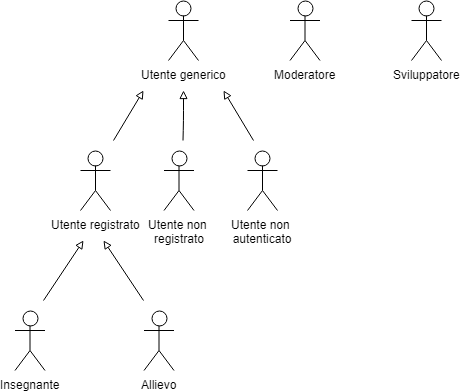
\includegraphics[scale=0.7]{images/attori.png}
			\caption{Attori del progetto}
		\end{figure}
		\newpage	
	\section{Casi d'uso}
		In questa sezione verranno elencati ed analizzati tutti i casi d'uso$^*$ individuati dal gruppo. Ogni caso d'uso verrà identificato da un codice univoco secondo le regole descritte nel documento \textit{Norme di progetto} e riportate di seguito. 
\subsection{Denominazione dei casi d'uso}
Ad ogni caso d'uso saranno associate le seguenti informazioni:
\begin{itemize}
\item il codice del requisito che lo interessa UC-[Codice];
\item un nome (univoco);
\item le pre-condizioni e le post-condizioni relative allo specifico caso d'uso;
\item gli attori coinvolti, sia primari che secondari;
\item lo scenario principale che il caso d'uso vorrebbe modellare;
\item le eventuali estensioni dello scenario principale.
\end{itemize}

\subsubsection{Gerarchie dei casi d'uso} 

Gli identificatori numerici assegnati a casi d'uso saranno organizzati gerarchicamente. Posto UC-X codice di un caso d'uso, allora UC-X.Y è figlio di UC-X ed esiste fra i due una relazione tra quelle elencate:
\begin{itemize}
\item UC-X.Y descrive nel dettaglio una delle funzionalita di UC-X;
\item UC-X.Y descrive una estensione (o scenario alternativo) dello scenario descritto in UC-X; 
\item UC-X.Y descrive una estensione dello scenario principale di due o più figli di UC-X.
\end{itemize}

\subsection{Elenco dei casi d'uso - Utente generico}
	\subsubsection{UC-13 Svolgimento esercizio}
	\begin{itemize}
			\item \textbf{Attori:} Utente generico.
			\item \textbf{Precondizione:}  L'allievo visualizza la vista per l'esecuzione dell'esercizio.
			\item \textbf{Postcondizione:} L'allievo visualizza la valutazione dell'esercizio.
			\item \textbf{Scenario principale:}
			\begin{enumerate}
				\item l'allievo compila i campi (UC-13.1).
				\item l'allievo conferma i dati inseriti.
				\item l'allievo visualizza la valutazione (UC-13.2).
			\end{enumerate}
	\end{itemize}
			
			\begin{figure}[h]
		\centering
		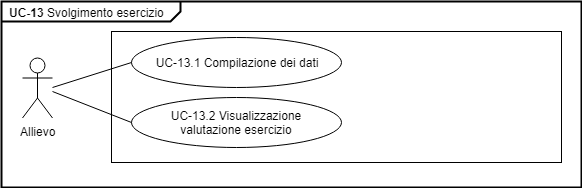
\includegraphics[scale=0.7]{images/UC-13.png}
		\caption{UC-13 Svolgimento esercizio}
	\end{figure}

	\subsubsection{UC-13.1 Compilazione dei campi}
		\begin{itemize}
			\item \textbf{Attori:} Utente generico.
			\item \textbf{Precondizione:} L'allievo ha selezionato un esercizio da eseguire.
			\item \textbf{Postcondizione:} L'allievo ha compilato i campi proposti dall'esercizio.
			\item \textbf{Scenario principale:}
				\begin{enumerate}
					\item L'allievo sceglie la classe grammaticale per ogni parola presentata.
					\item L'allievo conferma la soluzione dell'esercizio.
				\end{enumerate}
		\end{itemize}

	\subsubsection{UC-13.2 Visualizzazione della valutazione dell'esercizio}
	\begin{itemize}
			\item \textbf{Attori:} Utente generico.
			\item \textbf{Precondizione:} L'allievo ha completato l'esecuzione dell'esercizio.
			\item \textbf{Postcondizione:} L'allievo visualizza la valutazione dell'esercizio.
			\item \textbf{Scenario principale:}
				\begin{enumerate}
					\item l'allievo seleziona il correttore dell'esercizio(insegnante o algoritmo automatico).
					\item L'allievo visualizza la valutazione in base al correttore scelto.
				\end{enumerate}
	\end{itemize}				
			
	\subsubsection{UC-39 Inserimento di una frase da svolgere}
	\begin{itemize}
		\item \textbf{Attori:} Utente generico.
		\item \textbf{Precondizione:} L'allievo visualizza la vista principale dell'applicazione.
		\item \textbf{Postcondizione:} L'allievo visualizza la vista per l'esecuzione dell'esercizio.
		\item \textbf{Scenario principale:}
		\begin{enumerate}
			\item l'allievo scrive la frase da svolgere come esercizio
			\item l'allievo conferma la frase scelta
		\end{enumerate}
	\end{itemize}

	\subsubsection{UC-40 Selezione esercizio da svolgere}
	\begin{itemize}
			\item \textbf{Attori:} Utente generico.
			\item \textbf{Precondizione:} L'allievo visualizza la lista degli esercizi ricercati.
			\item \textbf{Postcondizione:} L'allievo visualizza la vista per l'esecuzione dell'esercizio.
			\item \textbf{Scenario principale:}
			\begin{enumerate}
					\item l'allievo seleziona la frase da svolgere.
					\item l'allievo conferma la selezione.
			\end{enumerate}
	\end{itemize}

	\subsubsection{UC-6 Ricerca esercizi}
		\begin{itemize}
			\item\textbf{ Attori:} Utente generico
			\item \textbf{Precondizione:} L'utente si trova nella vista principale dell'applicazione.
			\item \textbf{Postcondizione:} L'utente ottiene una lista degli esercizi filtrati.
			\item \textbf{Scenario principale:}
				\begin{enumerate}
					\item L'utente accede all'area dedicata alla ricerca degli esercizi.
					\item L'utente scrive la frase nella barra di ricerca.
					\item L'utente seleziona i filtri (UC-6.1).
					\item L'utente avvia la ricerca.
				\end{enumerate}
		\end{itemize}

	\subsubsection{UC-6.1 Filtraggio esercizi }
		\begin{itemize}
			\item \textbf{Attori:} Utente generico.
			\item \textbf{Precondizione:} L'utente si trova nella vista di ricerca degli esercizi dell'applicazione.
			\item \textbf{Postcondizione:} L'utente ha selezionato i filtri per la ricerca.
			\item \textbf{Scenario principale:}
				\begin{enumerate}
					\item L'utente può selezionare gli autori degli esercizi desiderati (UC-6.1.1)
					\item L'utente può selezionare il livello di difficoltà degli esercizi (UC-6.1.2).
					\item L'utente può selezionare gli argomenti degli esercizi (UC-6.1.3).
				\end{enumerate}
		\end{itemize}
		\begin{figure}[h]
			\centering
			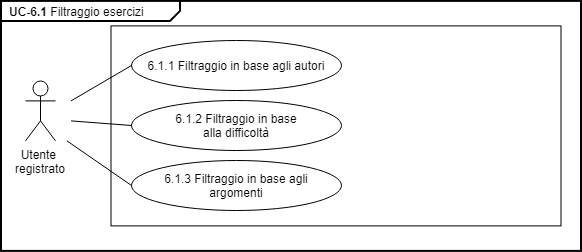
\includegraphics[scale=0.7]{images/UC-6.png}
			\caption{UC-6 Filtraggio esercizi}
		\end{figure}	

\subsubsection{UC-6.1.1 Filtraggio in base agli autori}
	\begin{itemize}
		\item \textbf{Attori:} Utente generico
		\item \textbf{Precondizione: } L'utente si trova nella vista di ricerca degli esercizi dell'applicazione
		\item \textbf{Postcondizione: } L'utente ha indicato gli autori nel filtro di ricerca 
		\item \textbf{Scenario principale:}
		\begin{enumerate}
			\item L'utente visualizza la lista degli autori
			\item L'utente seleziona gli autori di cui vuole vedere gli esercizi			
		\end{enumerate}
	\end{itemize}

\subsubsection{UC-6.1.2 Filtraggio in base alla difficoltà}
	\begin{itemize}
		\item \textbf{Attori:} Utente generico
		\item \textbf{Precondizione: } L'utente si trova nella vista di ricerca degli esercizi dell'applicazione
		\item \textbf{Postcondizione: } L'utente ha indicato la difficoltà nel filtro di ricerca 
		\item \textbf{Scenario principale:}
		\begin{enumerate}
			\item L'utente visualizza i livelli possibili di difficoltà (da 1 a 5)
			\item L'utente indica il livello di difficoltà degli esercizi cercati
		\end{enumerate}
	\end{itemize}

\subsubsection{UC-6.1.3 Filtraggio in base agli argomenti}
	\begin{itemize}
		\item \textbf{Attori:} Utente generico
		\item \textbf{Precondizione: } L'utente si trova nella vista di ricerca degli esercizi dell'applicazione
		\item \textbf{Postcondizione: } L'utente ha indicato gli autori nel filtro di ricerca 
		\item \textbf{Scenario principale:}
		\begin{enumerate}
			\item L'utente visualizza la lista degli argomenti (pronomi, verbi, aggettivi, articoli, avverbi, ecc..)
			\item L'utente seleziona gli argomenti di cui vuole vedere gli esercizi
		\end{enumerate}
	\end{itemize}

\subsubsection{UC-46 Segnalazione abuso di un esercizio}
	\begin{itemize}
		\item \textbf{Attori:} Utente generico
		\item \textbf{Precondizione:} L'utente si trova nella vista di svolgimento di un esercizio che ritiene non rispetti le norme di comportamento.
		\item \textbf{Postcondizione:} L'utente ha inviato una notifica di abuso del codice di comportamento
		\item \textbf{Scenario principale:}
		\begin{enumerate}
			\item L'utente seleziona l'opzione "Segnala abuso"
		\end{enumerate}
	\end{itemize}

\subsection{Elenco dei casi d'uso - Utente: utente non registrato}

\subsubsection{UC-1 Registrazione Allievo}
\begin{itemize}
		\item \textbf{Attori: }Utente non registrato.
		\item \textbf{Precondizione: }L'utente si trova nella vista di registrazione dell'applicazione.
		\item \textbf{Postcondizione: }L'utente è registrato come allievo.
		\item \textbf{Scenario principale: }
		\begin{enumerate}
		\item L'utente ha scelto di registrarsi al sistema, quindi di creare un nuovo profilo. 
		\item L'utente seleziona la tipologia allievo. 
		\item L'utente inserirà nome, cognome, username, email e password.
		\item L'utente fornirà il nome della scuola a cui appartiene e la città.
		\item L'utente conferma la registrazione.
		\end{enumerate}
		\item \textbf{Estensioni: }
		\begin{itemize}
			\item 5.a Nel caso in cui l'utente tenti l'inserimento di campi non validi vedrà comparire dei messaggi d'errore (UC-5).
		\end{itemize}
\end{itemize}
\begin{figure}[h]
	\centering
	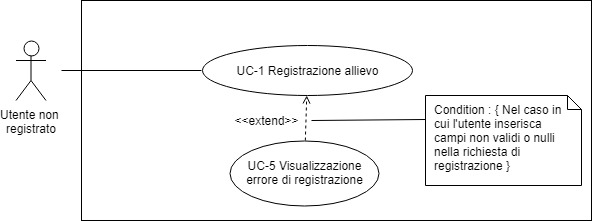
\includegraphics[scale=0.7]{images/UC-1_a.png}
	\caption{UC-1 Registrazione Allievo}
\end{figure}

\subsubsection{UC-33 Registrazione Insegnante}
\begin{itemize}
	\item \textbf{Attori: }Utente non registrato.
	\item \textbf{Precondizione: }L'utente si trova nella vista di registrazione dell'applicazione.
	\item \textbf{Postcondizione: }L'utente è in attesa di conferma.
	\item \textbf{Scenario principale: }
	\begin{enumerate}
		\item L'utente ha scelto di registrarsi al sistema, quindi di creare un nuovo profilo. 
		\item L'utente seleziona la tipologia insegnante. 
		\item L'utente inserirà nome, cognome, username, email e password.
		\item L'utente fornirà il nome della scuola a cui appartiene e la città.
		\item L'utente conferma la registrazione.
	\end{enumerate}
	\item \textbf{Estensioni: }
	\begin{itemize}
		\item 5.a Nel caso in cui l'utente tenti l'inserimento di campi non validi vedrà comparire dei messaggi d'errore (UC-5).
	\end{itemize}
\end{itemize}
\begin{figure}[h]
	\centering
	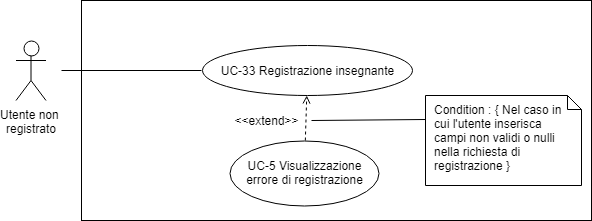
\includegraphics[scale=0.7]{images/UC-1i.png}
	\caption{UC-33 Registrazione Insegnante}
\end{figure}	

\subsubsection{UC-5 Visualizzazione errore di registrazione}
\begin{itemize}
	\item \textbf{Attori:} Utente non registrato
	\item \textbf{Precondizione:} L'utente ha confermato la richiesta di registrazione con campi non validi o nulli
	\item \textbf{Postcondizione:} L'utente torna alla vista di registrazione
	\item  \textbf{Scenario principale: }
	\begin{enumerate}
		\item Visualizza un messaggio di errore "Registrazione non avvenuta: campi non validi"
	\end{enumerate}
\end{itemize}

\subsubsection{UC-36 Notifica richiesta insegnante}
   \begin{itemize}
   \item \textbf{Attori:} Utente non registrato
   \item \textbf{Precondizione:} L'utente ha inviato la richiesta di registrazione come insegnante.
   \item \textbf{Postcondizione:} L'utente riceve la conferma di registrazione come insegnante. 
   \item \textbf{Scenario principale:}
    \begin{enumerate}
     \item L'utente riceve una notifica della conferma via e-mail.
    \end{enumerate}
  \end{itemize}

\subsection{Elenco dei casi d'uso - Utente: Utente non autenticato}

\subsubsection{UC-2 Autenticazione}
		\begin{itemize}
			\item \textbf{Attori:} Utente non autenticato.
			\item \textbf{Precondizione:} L'utente si trova nella vista di autenticazione dell'applicazione.
			\item \textbf{Postcondizione:} L'utente ha eseguito l'accesso con il proprio ruolo.
			\item \textbf{Scenario principale:}
				\begin{enumerate}
					\item L'utente inserisce la propria username e password.
					\item L'utente conferma l'accesso.
				\end{enumerate}
				\item \textbf{Estensioni:}
				\begin{itemize}
					\item 2.a Nel caso in cui l'utente tenti l'inserimento di campi non validi vedrà comparire messaggi d'errore (UC-34).
				\end{itemize}
		\end{itemize}
		
\subsubsection{UC-34 Visualizzazione errore di autenticazione}
		\begin{itemize}
			\item \textbf{Attori:} Utente non autenticato
			\item \textbf{Precondizione:} L'utente ha provato ad autenticarsi
			\item \textbf{Postcondizione:} L'utente torna alla vista di accesso alla piattaforma
			\item \textbf{Scenario principale:}
			\begin{enumerate}
				\item L'utente visualizza un messaggio di errore "Impossibile effettuare l'accesso: username o password errati"
			\end{enumerate}
		\end{itemize}
		
\subsection{Elenco dei casi d'uso - Utente: utente registrato}	
La categoria "utente registrato" comprende gli utenti registrati con i ruoli di allievo o insegnante.	
\subsubsection{UC-3 Modifica profilo}
		\begin{itemize}
			\item \textbf{Attori:} Utente registrato.
			\item \textbf{Precondizione:} L'utente si trova nella vista di modifica dei dati del proprio profilo.
			\item \textbf{Postcondizione:} L'utente ha modificato i propri dati personali.
			\item \textbf{Scenario principale:}
				\begin{enumerate}
					\item L'utente modifica username, password, scuola, città.
					\item L'utente conferma la modifica. 
				\end{enumerate}
				\item \textbf{Estensioni:}
				\begin{itemize}
					\item 2.a Nel caso in cui l'utente tenti l'inserimento di campi non validi vedrà comparire messaggi d'errore (UC-35).
				\end{itemize}
		\end{itemize}
		\begin{figure}[htbp]
			\centering
			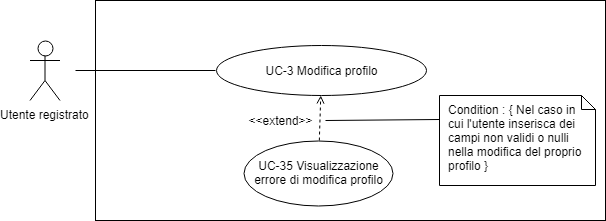
\includegraphics[scale=0.7]{images/UC-3.png}
			\caption{UC-3 Modifica profilo}
		\end{figure}
	
\subsubsection{UC-35 Visualizzazione errore di modifica del profilo}	
	\begin{itemize}
		\item \textbf{Attori:} Utente registrato
		\item \textbf{Precondizione:} L'utente ha inserito dei campi non validi o nulli nella modifica del proprio profilo
		\item \textbf{Postcondizione:} L'utente torna alla vista del proprio profilo
		\item \textbf{Scenario principale:}
		\begin{enumerate}
			\item L'utente visualizza un messaggio di errore "Modifica del profilo non avvenuta: campi non validi o nulli"
		\end{enumerate}
	\end{itemize}

\subsubsection{UC-31 Visualizza lista delle classi}		
\begin{itemize}
	\item \textbf{Attori:} Utente registrato.
	\item \textbf{Precondizione:} L'utente si trova nella vista principale del proprio profilo.
	\item \textbf{Postcondizione:} L'utente visualizza le classi che lo riguardano.
	\item \textbf{Scenario principale:}
	\begin{enumerate}
		\item L'utente seleziona l'opzione "vedi classi".
	\end{enumerate}		
\end{itemize}

\subsection{Elenco dei casi d'uso - Utente: moderatore}	
\subsubsection{UC-4 Verifica richiesta insegnante}
		\begin{itemize}
			\item \textbf{Attori:} Moderatore.
			\item \textbf{Precondizione:} Il moderatore si trova nella vista di amministrazione dell'applicazione.
			\item \textbf{Postcondizione:} Il moderatore ha confermato l'utente richiedente il ruolo di insegnante.
			\item \textbf{Scenario principale:}
				\begin{enumerate}
					\item Il moderatore visualizza la lista degli utenti che richiedono il ruolo di insegnante.
					\item Il moderatore accetta o rifiuta l'utente selezionato.
				\end{enumerate}
		\end{itemize}
		
\subsubsection{UC-23 Eliminazione di un esercizio}
			\begin{itemize}
			\item \textbf{Attori:} Moderatore.
			\item \textbf{Precondizione:} Il moderatore si trova nella vista di amministrazione dell'applicazione.
			\item \textbf{Postcondizione:} Il moderatore ha eliminato l'esercizio desiderato.
			\item \textbf{Scenario principale:}
				\begin{enumerate}
					\item Il moderatore indica l'esercizio da eliminare.
					\item Il moderatore conferma l'eliminazione dell'esercizio selezionato.
				\end{enumerate}
		\end{itemize}

\subsubsection{UC-8 Eliminazione di un utente}
\begin{itemize}
	\item \textbf{Attori:} Moderatore.
	\item \textbf{Precondizione:} Il moderatore si trova nella vista di amministrazione dell'applicazione.
	\item \textbf{Postcondizione:} Il moderatore ha eliminato l'utente desiderato.
	\item \textbf{Scenario principale:}
	\begin{enumerate}
		\item Il moderatore indica l'utente da eliminare.
		\item Il moderatore conferma l'eliminazione dell'utente selezionato.
	\end{enumerate}
\end{itemize}

\subsubsection{UC-47 Visualizzazione lista delle segnalazioni}
\begin{itemize}
	\item \textbf{Attori:} Moderatore.
	\item \textbf{Precondizione:} Il moderatore si trova nella vista di amministrazione dell'applicazione.
	\item \textbf{Postcondizione:} Il moderatore visualizza la lista delle segnalazioni ricevute.
	\item \textbf{Scenario principale:}
	\begin{enumerate}
		\item Il moderatore seleziona l'opzione "Lista delle segnalazioni"
	\end{enumerate}
\end{itemize}

\subsubsection{UC-48 Eliminazione segnalazione}
\begin{itemize}
	\item \textbf{Attori:} Moderatore.
	\item \textbf{Precondizione:} Il moderatore visualizza la lista delle segnalazioni ricevute.
	\item \textbf{Postcondizione:} Il moderatore ha eliminato la segnalazione desiderata.
	\item \textbf{Scenario principale:}
	\begin{enumerate}
		\item Il moderatore seleziona la segnalazione
		\item Il moderatore seleziona l'opzione "Elimina segnalazione"
	\end{enumerate}
\end{itemize}

\subsection{Elenco dei casi d'uso - Utente: insegnante}		
\subsubsection{UC-9 Modifica soluzione}
\begin{itemize}
\item \textbf{Attori:} Insegnante.
\item \textbf{Precondizione:} L'insegnante ha selezionato un esercizio di cui ha fornito una soluzione.
\item \textbf{Postcondizione:} La soluzione inserita è stata modificata.
\item \textbf{Scenario principale:}
		\begin{enumerate}
		\item L'insegnante visualizza le coppie (parola,classe grammaticale) con la vecchia soluzione.
		\item L'insegnante modifica le associazioni (parola,classe) che ritiene errate.
		\item L'insegnante conferma la modifica.
		\end{enumerate}
\end{itemize}

\subsubsection{UC-10 Visualizzazione esercizi inseriti}
\begin{itemize}
\item \textbf{Attori: }Insegnante.
		\item \textbf{Precondizione: }L'insegnante si trova nell'area del suo profilo.
		\item \textbf{Postcondizione: }L'insegnante visualizza una lista di esercizi inseriti. 
		\item \textbf{Scenario principale: }
		\begin{enumerate}
		\item L'insegnante accede alla vista degli esercizi inseriti.
		\end{enumerate}
	\end{itemize}
	
\subsubsection{UC-11 Eliminare una soluzione di un esercizio}
\begin{itemize}
\item \textbf{Attori: }Insegnante.
		\item \textbf{Precondizione: }L'insegnante ha selezionato la soluzione da eliminare.
		\item \textbf{Postcondizione: }La soluzione selezionata viene eliminata. 
		\item \textbf{Scenario principale: }
		\begin{enumerate}
		\item L'insegnante sceglie una soluzione da eliminare.
		\item L'insegnante conferma l'eliminazione.
		\end{enumerate}
\end{itemize}

\subsubsection{UC-12 Inserimento esercizio}
	\begin{itemize}
		\item \textbf{Attori: }Insegnante.
		\item \textbf{Precondizione: }L'insegnante è nella vista di inserimento di un nuovo esercizio.
		\item \textbf{Postcondizione: }L'esercizio è stato inserito.
		\item \textbf{Scenario principale: }
		\begin{enumerate} 
		\item L'insegnante inserisce la frase.
		\item L'insegnante inserisce la soluzione UC-12.1.
		\item L'insegnante inserisce gli argomenti UC-12.2.
		\item L'insegnante inserisce la difficoltà. UC-12.3
		\item L'insegnante conferma l'inserimento.
		\end{enumerate}
		\item \textbf{Estensioni:} 
		\begin{itemize}
		\item 1.a Nel caso in cui la frase inserita sia nulla, viene visualizzato un errore (UC-37).
		\end{itemize}
	\end{itemize}
	\begin{figure}[h]
		\centering
		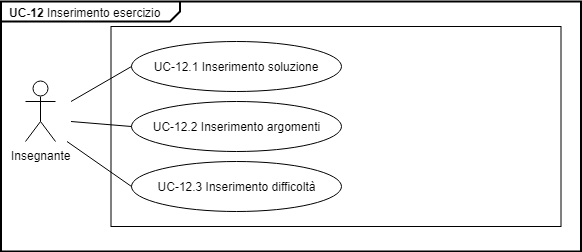
\includegraphics[scale=0.7]{images/UC-12.png}
		\caption{UC-12 Inserimento esercizio}
	\end{figure}

\subsubsection{UC-12.1 Inserimento di una soluzione}
\begin{itemize}
\item \textbf{Attori: }Insegnante.
\item \textbf{Precondizione: }L'insegnante è nella vista di inserimento di un nuovo esercizio.
\item \textbf{Postcondizione: }L'insegnante ha inserito la propria soluzione.
\item \textbf{Scenario principale: }
		\begin{enumerate} 
		\item L'insegnante visualizza la soluzione proposta dal generatore automatico. 
		\item L'insegnante può modificare le classi grammaticali assegnate dal generatore automatico che ritiene errate.
		\item L'insegnante seleziona lo stato della soluzione inserita, pubblica o privata.
		\item L'insegnante conferma la soluzione.
		\end{enumerate}	
\end{itemize}

\subsubsection{UC-12.2 Inserimento argomenti}
\begin{itemize}
\item \textbf{Attori: }Insegnante.

\item \textbf{Precondizione:} L'insegnante sta inserendo un esercizio, gli viene richiesta la compilazione di una lista di argomenti presenti nell'esercizio.
\item \textbf{Postcondizione:} L'insegnante ha selezionato gli argomenti trattati nell'esercizio.
\item \textbf{Scenario principale: }
		\begin{enumerate}
		\item L'insegnante visualizza la lista degli argomenti
		\item L'insegnante seleziona gli argomenti che vengono toccati nell'esercizio. 
		\end{enumerate}
\end{itemize}				

\subsubsection{UC-12.3 Inserimento della difficoltà}
\begin{itemize}
	\item \textbf{Attori: }Insegnante
	\item \textbf{Precondizione:} L'insegnante è nella vista di inserimento di un nuovo esercizio.
	\item \textbf{Postcondizione:} L'insegnante ha indicato il livello di difficoltà
	\item \textbf{Scenario principale:}
	\begin{enumerate}
		\item L'insegnante visualizza i livelli possibili di difficoltà (da 1 a 5)
		\item L'insegnante indica il livello di difficoltà dell'esercizio da inserire
	\end{enumerate}
\end{itemize}

\subsubsection{UC-37 Visualizzazione errore di inserimento di una frase vuota}
\begin{itemize}
	\item \textbf{Attori:} Insegnante
	\item \textbf{Precondizione:} L'insegnante è nella vista di inserimento di un nuovo esercizio e ha inserito una frase vuota.
	\item \textbf{Postcondizione:} L'insegnante torna alla vista di inserimento dell'esercizio.
	\item \textbf{Scenario principale:}
	\begin{enumerate}
		\item L'insegnante visualizza un messaggio di errore "La frase inserita è vuota"
	\end{enumerate}
\end{itemize}

\subsubsection{UC-24 Creazione classe}
\begin{itemize}
	\item \textbf{Attori:} Insegnante.
	\item \textbf{Precondizione:} L'insegnante si trova nella vista principale dell'applicazione.
	\item \textbf{Postcondizione:} L'insegnante si trova nella vista di gestione della classe creata.
	\item \textbf{Scenario principale:}
	\begin{enumerate}
		\item L'insegnante selezione l'opzione "aggiungi classe".
		\item L'insegnante assegna un nome alla classe.
		\item L'insegnante assegna una descrizione alla classe.
		\item L'insegnante conferma la creazione.
	\end{enumerate}
\end{itemize}

\subsubsection{UC-25 Eliminare una classe}
\begin{itemize}
	\item \textbf{Attori:} Insegnante.
	\item \textbf{Precondizione:} L'insegnante si trova nella vista di gestione di una propria classe.
	\item \textbf{Postcondizione:} L'insegnante elimina la classe dal sistema.
	\item \textbf{Scenario principale:}
	\begin{enumerate}
		\item l'insegnante clicca sul pulsante di eliminazione della classe.
		\item l'insegnante conferma l'eliminazione.
	\end{enumerate}
\end{itemize}

\subsubsection{UC-26 Inserimento alunni}
\begin{itemize}
	\item \textbf{Attori:} Insegnante.
	\item \textbf{Precondizione:} L'insegnante si trova nella vista di gestione di una propria classe.
	\item \textbf{Postcondizione:} L'insegnante visualizza gli alunni inseriti.
	\item \textbf{Scenario principale:}
	\begin{enumerate}
		\item L'insegnante seleziona l'opzione di aggiunta.
		\item L'insegnante indica gli studenti da aggiungere (UC-26.1).
		\item L'insegnante conferma l'inserimento.
	\end{enumerate}
\end{itemize}

\subsubsection{UC-26.1 Selezione alunni per l'inserimento}
\begin{itemize}
	\item \textbf{Attori:} Insegnante
	\item \textbf{Precondizione:} l'insegnante si trova nella vista di aggiunta degli alunni a una classe
	\item \textbf{Postcondizione:} l'insegnante ha indicato gli alunni da inserire nella classe
	\item \textbf{Scenario principale:}
	\begin{enumerate}
		\item l'insegnante visualizza la lista di tutti gli alunni presenti sulla piattaforma
		\item l'insegnante ricerca gli alunni da inserire (UC-26.1.1)	
		\item l'insegnante seleziona gli alunni da inserire
	\end{enumerate}
\end{itemize}

\subsubsection{UC-26.1.1 Ricerca alunno}
\begin{itemize}
	\item \textbf{Attori:} Insegnante
	\item \textbf{Precondizione:} l'insegnante visualizza la lista di tutti gli alunni presenti sulla piattaforma
	\item \textbf{Postcondizione:} l'insegnante visualizza l'username dell'alunno cercato
	\item \textbf{Scenario principale:}
	\begin{enumerate}
		\item l'insegnante scrive l'username, o una sua parte, di un alunno
	\end{enumerate}
\end{itemize}

\subsubsection{UC-27 Assegnazione esercizi}
\begin{itemize}
	\item \textbf{Attori:} Insegnante.
	\item \textbf{Precondizione:} Visualizza una lista di esercizi da una ricerca eseguita
	\item \textbf{Postcondizione:} L'insegnante ha assegnato esercizi alla classe.
	\item \textbf{Scenario principale:}
	\begin{enumerate}
		\item l'insegnante seleziona degli esercizi in lista da assegnare.
		\item l'insegnante indica la classe a cui assegnarli
		\item l'insegnante conferma l'assegnazione
	\end{enumerate}
\end{itemize}

\subsubsection{UC-30 Visualizza lista degli alunni iscritti nella classe}		
\begin{itemize}
	\item \textbf{Attori:} Insegnante.
	\item \textbf{Precondizione:} L'insegnante si trova nella vista di gestione di una propria classe.
	\item \textbf{Postcondizione:} L'insegnante visualizza l'elenco degli alunni iscritti.
	\item \textbf{Scenario principale:}
	\begin{enumerate}
		\item L'insegnante seleziona l'opzione "vedi alunni".
	\end{enumerate}		
\end{itemize}

\subsubsection{UC-28 Visualizzare i progressi di un alunno della classe}
\begin{itemize}
	\item \textbf{Attori:} Insegnante.
	\item \textbf{Precondizione}: L'insegnante visualizza l'elenco degli alunni iscritti alla classe.
	\item \textbf{Postcondizione:} L'insegnante visualizza i progressi relativi allo studente selezionato.
	\item \textbf{Scenario principale:}
	\begin{enumerate}
		\item l'insegnante seleziona lo studente trovato
		\item l'insegnante visualizza i grafici che riportano la media totale, la media per tipologia di esercizi e lo sviluppo della media nel tempo
	\end{enumerate}
\end{itemize}

\subsubsection{UC-29 Elimina alunno dalla classe}		
\begin{itemize}
	\item \textbf{Attori:} Insegnante.
	\item \textbf{Precondizione:} L'insegnante visualizza la lista degli alunni della classe.
	\item \textbf{Postcondizione:} L'insegnante ha rimosso l'allievo dalla classe.
	\item \textbf{Scenario principale:}
	\begin{enumerate}
		\item L'insegnante seleziona l'allievo da rimuovere dalla classe.
		\item L'insegnante conferma l'eliminazione.
	\end{enumerate}	
\end{itemize}


\subsection{Elenco dei casi d'uso - Utente: allievo}

	\subsubsection{UC-14 Visualizzazione progressi}
	\begin{itemize}
			\item \textbf{Attori:} Allievo.
			\item \textbf{Precondizione:} L'allievo si trova nella vista del proprio profilo.
			\item \textbf{Postcondizione:} L'allievo visualizza i progressi svolti fino a quel momento.
			\item \textbf{Scenario principale:}
				\begin{enumerate}
					\item L'allievo visualizza la media delle valutazioni ricevute, la media per tipologia di esercizi e lo sviluppo della media nel tempo
				\end{enumerate}
	\end{itemize}
	
	\subsubsection{UC-7 Visualizzazione lista delle classi di appartenenza}
		\begin{itemize}
			\item \textbf{Attori:} Allievo
			\item \textbf{Precondizione:} L'allievo si trova nella vista del proprio profilo
			\item \textbf{Postcondizione:} L'allievo visualizza la lista delle classi a cui appartiene
			\item \textbf{Scenario principale:}
			\begin{enumerate}
				\item L'allievo seleziona l'opzione "Lista delle classi"
			\end{enumerate}
		\end{itemize}			

	\subsubsection{UC-32 Annullamento dell'iscrizione a una classe}
		\begin{itemize}
			\item \textbf{Attori:} Allievo
			\item \textbf{Precondizione:} L'allievo visualizza la lista delle classi a cui appartiene
			\item \textbf{Postcondizione:} L'allievo ha annullato l'iscrizione alla classe
			\item \textbf{Scenario principale:}
			\begin{enumerate}
				\item L'allievo seleziona l'opzione "Disiscriviti"
			\end{enumerate}
		\end{itemize}					
		
		
	\subsubsection{UC-45 Visualizzazione delle informazioni della classe}
		\begin{itemize}
			\item \textbf{Attori:} Allievo
			\item \textbf{Precondizione:} L'allievo visualizza la lista delle classi a cui appartiene
			\item \textbf{Postcondizione:} L'allievo visualizza le informazioni della classe indicata (allievi iscritti e media delle valutazioni)
			\item \textbf{Scenario principale:}
			\begin{enumerate}
				\item L'allievo seleziona una classe
			\end{enumerate}
		\end{itemize}
		\subsection{Elenco dei casi d'uso - Utente: sviluppatore}	

\subsubsection{UC-15 Ricerca dei dati delle annotazioni}
		\begin{itemize}
			\item \textbf{Attori:} Sviluppatore.
			\item \textbf{Precondizione:} Lo sviluppatore si trova nella vista principale dell'applicazione.
			\item \textbf{Postcondizione:} Lo sviluppatore ottiene una lista delle annotazioni correnti delle frasi.
			\item \textbf{Scenario principale:}
				\begin{enumerate}
					\item Lo sviluppatore accede all'area dei dati.
					\item Lo sviluppatore scrive nella barra di ricerca una sottostringa della frase cercata.
					\item lo sviluppatore seleziona i filtri da usare nella ricerca (UC-15.1).
					\item lo sviluppatore conferma la ricerca
				\end{enumerate}
		\end{itemize}
	
	\subsubsection{UC-15.1 Filtraggio dei dati}	
		\begin{itemize}
			\item \textbf{Attori:} Sviluppatore.
			\item \textbf{Precondizione:} Lo sviluppatore si trova nell'area dati e ha scritto nella barra di ricerca una sottostringa della frase cercata.
			\item \textbf{Postcondizione:} Lo sviluppatore ha indicato i filtri da applicare alla ricerca.
			\item \textbf{Scenario principale:}
				\begin{enumerate}
					\item Lo sviluppatore seleziona il filtro su base temporale (UC-15.1.1).
					\item Lo sviluppatore seleziona il filtro in base agli utenti (UC-15.1.2).
				\end{enumerate}
			\end{itemize}
	\begin{figure}[h]
			\centering
			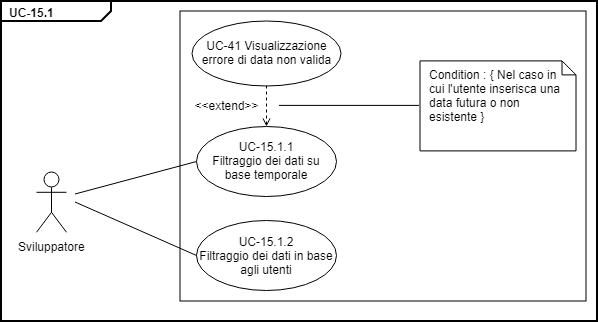
\includegraphics[scale=0.7]{images/UC-15_1.png}
			\caption{UC-15.1 Filtraggio dei dati}
		\end{figure}	
	
	\subsubsection{UC-15.1.1 Filtraggio dei dati su base temporale}	
		\begin{itemize}
			\item \textbf{Attori:} Sviluppatore.
			\item \textbf{Precondizione:} Lo sviluppatore si trova nell'area dati e ha scritto nella barra di ricerca una sottostringa della frase cercata.
			\item \textbf{Postcondizione:} Lo sviluppatore ha indicato il filtro su base temporale della ricerca.
			\item \textbf{Scenario principale:}
				\begin{enumerate}
					\item Lo sviluppatore indica due date che definiscono un intervallo di tempo per restringere la ricerca.
				\end{enumerate}
			\item \textbf{Estensioni:}
				\begin{itemize}
					\item 4.a Se i parametri inseriti dall'utente non sono coerenti viene mostrato un messaggio di errore (UC-41).
				\end{itemize}		
		\end{itemize}
			
	\subsubsection{UC-41 Visualizzazione errore di data non valida}
		\begin{itemize}					
			\item \textbf{Attori:} Sviluppatore.
			\item \textbf{Precondizione:} Lo sviluppatore ha indicato un intervallo di tempo non valido.
			\item \textbf{Postcondizione:} Lo sviluppatore torna all'area dati.
			\item \textbf{Scenario principale:}
				\begin{enumerate}
					\item Lo sviluppatore visualizza un messaggio di errore "L'intervallo di tempo indicato non è valido".
				\end{enumerate}	
		\end{itemize}					
						
	\subsubsection{UC-15.1.2 Filtraggio dei dati in base agli utenti}	
		\begin{itemize}
			\item \textbf{Attori:} Sviluppatore.
			\item \textbf{Precondizione:} Lo sviluppatore si trova nell'area dati e ha scritto nella barra di ricerca una sottostringa della frase cercata.
			\item \textbf{Postcondizione:} Lo sviluppatore ha indicato il filtro in base agli utenti.
			\item \textbf{Scenario principale:}
				\begin{enumerate}
					\item Lo sviluppatore indica l'inclusione o l'esclusione di un utente.
					\item Lo sviluppatore indica gli utenti da includere o escludere.
				\end{enumerate}
		\end{itemize}
		
	\subsubsection{UC-16 Visualizzazione dei dati di una annotazione di una frase}
		\begin{itemize}
			\item \textbf{Attori:} Sviluppatore.
			\item \textbf{Precondizione:} Lo sviluppatore si trova nell'area dati e ha a disposizione i risultati della ricerca delle annotazioni.
			\item \textbf{Postcondizione:} Lo sviluppatore legge i dati di una annotazione di una frase.
			\item \textbf{Scenario principale:}
				\begin{enumerate}
					\item Lo sviluppatore seleziona una annotazione.
					\item Lo sviluppatore visualizza data, utente e soluzione proposta
				\end{enumerate}
		\end{itemize}
	
	\subsubsection{UC-17 Visualizzazione storico}		
		\begin{itemize}
			\item \textbf{Attori:} Sviluppatore.
			\item \textbf{Precondizione:} Lo sviluppatore si trova nell'area dati e ha a disposizione i risultati della ricerca delle annotazioni.
			\item \textbf{Postcondizione:} Lo sviluppatore visualizza lo storico delle annotazioni ottenute dalla ricerca precedente.
			\item \textbf{Scenario principale:}
			\begin{enumerate}
				\item Lo sviluppatore seleziona l'opzione "vedi storico".
			\end{enumerate}
		\end{itemize}	
		
	\subsubsection{UC-18 Ordinamento dei risultati}
		\begin{itemize}
			\item \textbf{Attori:} Sviluppatore.
			\item \textbf{Precondizione:} Lo sviluppatore si trova nell'area dati con i risultati della ricerca effettuata.
			\item \textbf{Postcondizione:} Lo sviluppatore ottiene la lista precedente ordinata in base alle scelte effettuate.
			\item \textbf{Scenario principale:}
				\begin{enumerate}
					\item Lo sviluppatore sceglie il parametro secondo il quale ordinare i risultati (alfabetico, frequenza, ultima correzione, utente).
					\item Lo sviluppatore conferma l'ordinamento scelto.
				\end{enumerate}
		\end{itemize} 
	
	\subsubsection{UC-19 Download dei dati raccolti}
		\begin{itemize}
			\item \textbf{Attori:} Sviluppatore.
			\item \textbf{Precondizione:} Lo sviluppatore si trova nell'area dati con i risultati della ricerca effettuata.
			\item \textbf{Postcondizione:} Lo sviluppatore ottiene un file \texttt{.txt} con i dati dei risultati precedentemente trovati.
			\item \textbf{Scenario principale:}
				\begin{enumerate}
					\item Lo sviluppatore richiede il download dei dati.
					\item Lo sviluppatore decide il path in cui il file viene salvato.
					\item Lo sviluppatore esegue il salvataggio.
				\end{enumerate}
			\item \textbf{Estensioni:}
				\begin{itemize}
					\item 2.a Se il path indicato è inesistente, viene visualizzato un messaggio di errore (UC-42).
				\end{itemize}
		\end{itemize}
		\begin{figure}[h]
			\centering
			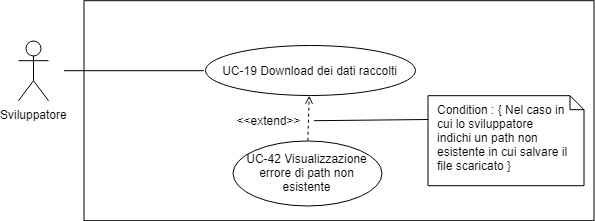
\includegraphics[scale=0.7]{images/UC-19.png}
			\caption{UC-19 Download dei dati raccolti}
		\end{figure}	

	\subsubsection{UC-42 Visualizzazione errore di path inesistente}
		\begin{itemize}					
			\item \textbf{Attori:} Sviluppatore.
			\item \textbf{Precondizione:} Lo sviluppatore ha indicato un path non esistente.
			\item \textbf{Postcondizione:} Lo sviluppatore torna all'area dati.
			\item \textbf{Scenario principale:}
				\begin{enumerate}
					\item Lo sviluppatore visualizza un messaggio di errore "Path inesistente".
				\end{enumerate}	
		\end{itemize}				
				
	\subsubsection{UC-20 Download di un dataset}
		\begin{itemize}
			\item \textbf{Attori:} Sviluppatore.
			\item \textbf{Precondizione:} Lo sviluppatore si trova nell'area dati con i risultati della ricerca effettuata.
			\item \textbf{Postcondizione:} Lo sviluppatore ottiene il dataset in un file \texttt{.txt}.
			\item \textbf{Scenario principale:}
			\begin{enumerate}
				\item Lo sviluppatore richiede il download del dataset, contenente l'input della fase di train del software di apprendimento automatico.
				\item Lo sviluppatore decide il path in cui il file viene salvato.
				\item Lo sviluppatore esegue il salvataggio.
			\end{enumerate}
			\item \textbf{Estensioni:}
				\begin{itemize}
					\item 2.a Se il path indicato è inesistente, viene visualizzato un messaggio di errore (UC-42).
				\end{itemize}
		\end{itemize}
	
	\subsubsection{UC-21 Download di un modello}
		\begin{itemize}
			\item \textbf{Attori:} Sviluppatore.
			\item \textbf{Precondizione:} Lo sviluppatore si trova nella vista con le informazioni del modello selezionato.
			\item \textbf{Postcondizione:} Lo sviluppatore ottiene un file binario con il modello.
			\item \textbf{Scenario principale:}
			\begin{enumerate}
					\item Lo sviluppatore richiede il download del modello.
					\item Lo sviluppatore decide il path in cui il file viene salvato.
					\item Lo sviluppatore esegue il salvataggio.
				\end{enumerate}
			\item \textbf{Estensioni:}
				\begin{itemize}
					\item 2.a Se il path indicato è inesistente, viene visualizzato un messaggio di errore (UC-42).
				\end{itemize}
		\end{itemize}	
		
	\subsubsection{UC-22 Creazione di un modello}		
		\begin{itemize}
			\item \textbf{Attori:} Sviluppatore.
			\item \textbf{Precondizione:} Lo sviluppatore si trova nell'area dati.
			\item \textbf{Postcondizione:} Lo sviluppatore aggiunge un modello alla piattaforma.
			\item \textbf{Scenario principale:}
			\begin{enumerate}
				\item Lo sviluppatore seleziona la funzione di aggiunta di un modello.
				\item Lo sviluppatore inserisce il file che contiene un dataset.
				\item Lo sviluppatore conferma la creazione.
			\end{enumerate}
			\item \textbf{Estensioni:}
				\begin{itemize}
					\item 4.a Se il dataset fornito ha un formato errato, viene visualizzato un messaggio di errore (UC-43).
				\end{itemize}
		\end{itemize}
		
		\begin{figure}[h]
			\centering
			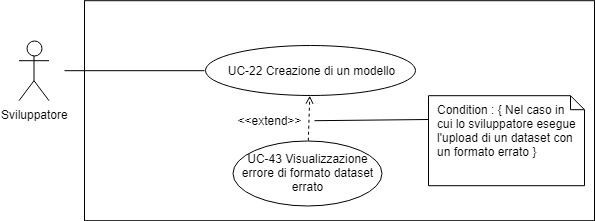
\includegraphics[scale=0.7]{images/UC-22.png}
				\caption{UC-22 Creazione di un modello}
		\end{figure}	
	
	\subsubsection{UC-43 Visualizzazione errore di formato del dataset errato}	
	\begin{itemize}					
			\item \textbf{Attori:} Sviluppatore.
			\item \textbf{Precondizione:} Lo sviluppatore ha fornito un formato dataset non corretto.
			\item \textbf{Postcondizione:} Lo sviluppatore torna all'area dati.
			\item \textbf{Scenario principale:}
				\begin{enumerate}
					\item Lo sviluppatore visualizza un messaggio di errore "Formato dataset non corretto".
				\end{enumerate}	
		\end{itemize}		
	
	\subsubsection{UC-44 Cambio modello}
	\begin{itemize}					
			\item \textbf{Attori:} Sviluppatore.
			\item \textbf{Precondizione:} Lo sviluppatore si trova nell'area dati.
			\item \textbf{Postcondizione:} Lo sviluppatore ha cambiato il modello utilizzato dal softwere di apprendimento automatico.
			\item \textbf{Scenario principale:}
				\begin{enumerate}
				\item Lo sviluppatore seleziona la funzione di cambio modello.
				\item Lo sviluppatore seleziona il modello che vuole utilizzare da una lista di modelli caricati o creati precedentemente.
				\item Lo sviluppatore conferma le modifiche. 
				\end{enumerate}	
		\end{itemize}		
	
		\newpage	
	\section{Requisiti}
		\section{Resoconto attività di verifica}
\subsection{Prodotto}
\subsubsection{Documentazione}
Nella tabella seguente vengono riportati i risultati delle verifiche eseguite sui documenti. Il resoconto contiene le verifiche sia dei documenti esterni, cioè utili al committente, sia interni, utili invece al team Ottobit.\\
{\renewcommand{\arraystretch}{1.5}%
\begin{longtable}{>{\centering\arraybackslash}m{3cm} >{\centering\arraybackslash}m{4cm} >{\centering\arraybackslash}m{5cm} >{\centering\arraybackslash}m{2cm}}
	\rowcolor{LightBlue}
		  \textbf{\textcolor{white}{Data}}
		& \textbf{\textcolor{white}{Autore}}
		& \textbf{\textcolor{white}{Documento}} 
		& \textbf{\textcolor{white}{Versione}}\\
		2019-01-11
		& Gianmarco Pettenuzzo
		& \textit{Analisi dei requisiti}
		& 0.1.0\\
		\rowcolor{LightGray}
		\multicolumn{4}{p{15.25cm}}{\textbf{Descrizione:} 
			Documento corretto e pronto per l'approvazione.
		}\\
		\rowcolor{LightGray}
		\multicolumn{4}{p{15.25cm}}{
			\textbf{Indice di Gulpease:} 82
		}\\
		\rowcolor{LightGray}
		\multicolumn{4}{p{15.25cm}}{
			\textbf{Esito:} Accettato
		}\\
		\hline
		2019-01-11
		& Giovanni Bergo
		& \textit{Piano di qualifica}
		& 0.2.0\\
		\rowcolor{LightGray}
		\multicolumn{4}{p{15.25cm}}{\textbf{Descrizione:} 
			Documento conforme e senza particolari errori da evidenziare.
		}\\
		\rowcolor{LightGray}
		\multicolumn{4}{p{15.25cm}}{
			\textbf{Indice di Gulpease:} 72
		}\\
		\rowcolor{LightGray}
		\multicolumn{4}{p{15.25cm}}{
			\textbf{Esito:} Accettato
		}\\
		\hline
		
		2018-01-11
		& Giovanni Peron
		& \textit{Piano di progetto}
		& 0.4.0\\
		\rowcolor{LightGray}
		\multicolumn{4}{p{15.25cm}}{\textbf{Descrizione:} 
			Nessun problema da segnalare.
		}\\
		\rowcolor{LightGray}
		\multicolumn{4}{p{15.25cm}}{
			\textbf{Indice di Gulpease:} 64
		}\\
		\rowcolor{LightGray}
		\multicolumn{4}{p{15.25cm}}{
			\textbf{Esito:} Accettato
		}\\
		\hline
		
		2018-01-10
		& Giovanni Peron
		& \textit{Piano di progetto}
		& 0.3.0\\
		\rowcolor{LightGray}
		\multicolumn{4}{p{15.25cm}}{\textbf{Descrizione:} 
			Nella sezione §4.1.2 sotto il paragrafo Analisi dei requisiti (2018-12-19 - 2018-02-09) da ricontrollare  il corsivo dei riferimenti ai documenti. Nel capitolo §4 posizione delle caption delle tabelle da uniformare. Mancanti le caption nelle ultime sei tabelle del documento.
		}\\
		\rowcolor{LightGray}
		\multicolumn{4}{p{15.25cm}}{
			\textbf{Indice di Gulpease:} 64
		}\\
		\rowcolor{LightGray}
		\multicolumn{4}{p{15.25cm}}{
			\textbf{Esito:} Non accettato
		}\\
		\hline
		
		2018-12-28
		& Giovanni Bergo
		& \textit{Piano di qualifica}
		& 0.1.0\\
		\rowcolor{LightGray}
		\multicolumn{4}{p{15.25cm}}{\textbf{Descrizione:} 
		Footer mancante. Piccoli errori grammaticali e di punteggiatura. Completamento descrizione §1.3 Note esplicative. Url citazioni non collegati al sito web. Introdurre rifermento a sezioni come indicato nelle 	
		textit{Norme di progetto}. Elenco delle tabelle e figure mancanti.
		}\\
		\rowcolor{LightGray}
		\multicolumn{4}{p{15.25cm}}{
			\textbf{Indice di Gulpease:} 66
		}\\
		\rowcolor{LightGray}
		\multicolumn{4}{p{15.25cm}}{
			\textbf{Esito:} Non accettato
		}\\
		\hline
		
		2018-12-26
		& Michele Bortone
		& \textit{Norme di progetto}
		& 0.2.0\\
	\rowcolor{LightGray}
	\multicolumn{4}{p{15.25cm}}{\textbf{Descrizione:} 
	Documento conforme e senza particolari errori da evidenziare.
	Pronto per l'approvazione.
	}\\
	\rowcolor{LightGray}
	\multicolumn{4}{p{15.25cm}}{
	\textbf{Indice di Gulpease:} 67
	}\\
	\rowcolor{LightGray}
	\multicolumn{4}{p{15.25cm}}{
	\textbf{Esito:} Accettato
	}\\
	\hline
		2018-12-18
		& Giovanni Peron
		& \textit{Piano di progetto}
		& 0.2.0\\
		\rowcolor{LightGray}
	\multicolumn{4}{p{15.25cm}}{\textbf{Descrizione:} Nulla da segnalare.
	}\\
	\rowcolor{LightGray}
	\multicolumn{4}{p{15.25cm}}{
	\textbf{Indice di Gulpease:} 63
	}\\
		\rowcolor{LightGray}
	\multicolumn{4}{p{15.25cm}}{
	\textbf{Esito:} Accettato
	}\\
		\hline
				2018-12-16
		& Michele Bortone
		& \textit{Studio di fattibilità}
		& 0.2.0\\
		\rowcolor{LightGray}
	\multicolumn{4}{p{15.25cm}}{\textbf{Descrizione:} 
	Nulla da segnalare.
	}\\
	\rowcolor{LightGray}
	\multicolumn{4}{p{15.25cm}}{
	\textbf{Indice di Gulpease:} 60
	}\\
		\rowcolor{LightGray}
	\multicolumn{4}{p{15.25cm}}{
	\textbf{Esito:} Accettato
	}\\
	\hline
		2018-12-16
		& Giovanni Peron
		& \textit{Piano di progetto}
		& 0.1.0\\
		\rowcolor{LightGray}
	\multicolumn{4}{p{15.25cm}}{\textbf{Descrizione:} Nella tabella del'analisi dei rischi del capitolo §2 ci sono ripetizioni nelle righe R01 e T01 entrambe nella colonna rilevamento. Il contenuto della tabella risulta tagliato a fine pagina 4. In §3.1 a riga 6 suggerisco di inserire Proof of Concept nel glossario. In tutto il documento rivedere il formato delle date secondo le norme di progetto. Per informazioni più dettagliate vedi i commenti scritti nel file relativo al documento.
	}\\
	\rowcolor{LightGray}
	\multicolumn{4}{p{15.25cm}}{
	\textbf{Indice di Gulpease:} 67
	}\\
		\rowcolor{LightGray}
	\multicolumn{4}{p{15.25cm}}{
	\textbf{Esito:} Non accettato
	}\\
		\hline
		2018-12-16
		& Michele Bortone
		& \textit{Norme di progetto}
		& 0.1.0\\
		\rowcolor{LightGray}
	\multicolumn{4}{p{15.25cm}}{\textbf{Descrizione:} 
	Il correttore segnala alcuni errori ortografici.
	Sezione §1 incompleta.
	Sezione §2.1 incompleta.
	Nella sezione §4.1.3.5 è presente un errore nella descrizione delle norme riguardanti l'inserimento delle figure all'interno di un documento. Suggerisco di aggiungere l'obbligo di inserire una breve didascalia dell'immagine corrispondente.
	Nella sezione §5.1.4 è presente un errore riguardo i compiti di ciascun ruolo. Bisogna correggere il redattore dello Studio di fattibilità.
	}\\
	\rowcolor{LightGray}
	\multicolumn{4}{p{15.25cm}}{
	\textbf{Indice di Gulpease:}74
	}\\
		\rowcolor{LightGray}
	\multicolumn{4}{p{15.25cm}}{
	\textbf{Esito:} Non accettato
	}\\
	\hline
		2018-12-16
		& Michele Bortone
		& \textit{Studio di fattibilità}
		& 0.1.0\\
	\rowcolor{LightGray}
	\multicolumn{4}{p{15.25cm}}{\textbf{Descrizione:} 
	Il correttore segnala alcuni errori ortografici.
	Elenchi puntati non conformi alle \textit{Norme di progetto}.
	}\\
	\rowcolor{LightGray}
	\multicolumn{4}{p{15.25cm}}{
	\textbf{Indice di Gulpease:} 58
	}\\
		\rowcolor{LightGray}
	\multicolumn{4}{p{15.25cm}}{
	\textbf{Esito:} Non accettato
	}\\\hline
	
	\caption{Resoconto attività di verifica}
\end{longtable}
}
\subsubsection{Test di sistema}
Di seguito riportiamo una tabella contenente i test di sistema che intendiamo implementare per la verifica dei requisiti funzionali specificati nell'\emph{Analisi dei requisiti}.
{\renewcommand{\arraystretch}{2}%
\begin{longtable}{|>{\centering\arraybackslash}m{1.6cm}|>{\centering\arraybackslash}m{1.7cm}|m{6.41cm}|>{\centering\arraybackslash}m{3.1cm}|}		
	\rowcolor{LightBlue}
		\textbf{\textcolor{white}{Codice\newline test}}
		& \textbf{\textcolor{white}{Codice\newline requisito}}
		& \multicolumn{1}{|c|}{\textbf{\textcolor{white}{ Descrizione}}}
		& \textbf{\textcolor{white}{Stato}}\\

		\hline
		\rowcolor{LightGray}
		TS-RO1
		& ROF1 
		& Verifica che l'utente riesca a registrarsi alla piattaforma creando un account personale. 
		& non implementato\\ \hline
		\rowcolor{white}
		TS-RO2
		& ROF2 
		& Verifica che l'utente possa eseguire l'accesso alla piattaforma utilizzando le sue credenziali.
		& non implementato\\ \hline
		\rowcolor{LightGray}
		TS-RD1
		& RDF1 
		& Verifica che l'utente possa modificare i dati del proprio profilo personale.
		& non implementato\\ \hline
		\rowcolor{white}
		TS-RD2
		& RDF2 
		& Verifica che l'amministratore possa verificare le credenziali di un utente che richiede la registrazione come insegnante. 
		& non implementato\\ \hline
		\rowcolor{LightGray}
		TS-RD3
		& RDF3 
		& Verifica che l'utente venga avvisato in caso di errore nell'inserimento dei dati richiesti.
		& non implementato\\ \hline
		\rowcolor{white}
		TS-RO3		
		& ROF3 
		& Verifica che l'insegnante e l'allievo possano ricercare degli esercizi sulla piattaforma.
		& non implementato\\ \hline
		\rowcolor{LightGray}
		TS-RP1		
		& RPF1 
		& Verifica che durante la ricerca, l'utente abbia la possibilità di impostare dei filtri per raffinarla. 		
		& non implementato\\ \hline
		\rowcolor{white}
		TS-RD4		
		& RDF4 
		& Verifica che dopo una ricerca, l'utente venga avvisato con un messaggio nel caso in cui il sistema non abbia trovato nessun risultato corrispondente ai criteri selezionati.
		& non implementato\\ \hline
		\rowcolor{LightGray}
		TS-RP2		
		& RPF2 
		& Verifica che l'amministratore possa eliminare un utente iscritto alla piattaforma.
		& non implementato\\ \hline
		\rowcolor{white}
		TS-RP3		
		& RPF3 
		& Verifica che l'insegnante possa modificare una soluzione di un esercizio da lui fornita
		& non implementato\\ \hline
		\rowcolor{LightGray}
		TS-RD5		
		& RDF5 
		& Verifica che l'insegnante, accedendo alla sua area del profilo, possa visualizzare la lista degli esercizi da lui creati. 
		& non implementato\\ \hline
		\rowcolor{white}
		TS-RP4		
		& RPF4 
		& Verifica che l'insegnante possa eliminare una soluzione di un esercizio da lui fornita. 
		& non implementato\\ \hline
		\rowcolor{LightGray}
		TS-RP5		
		& RPF5 
		& Verifica che l'insegnante possa indicare gli argomenti trattati nell'esercizio in fase di creazione.
		& non implementato\\ \hline
		\rowcolor{white}
		TS-RO4		
		& ROF4 
		& Verifica che l'allievo possa inserire una frase da svolgere o selezionare un esercizio da quelli disponibili sul sistema.
		& non implementato\\ \hline
		\rowcolor{LightGray}
		TS-RO5		
		& ROF5 
		& Verifica che l'allievo possa compilare i campi relativi alle parole della frase al fine di completare l'esercizio selezionato.
		& non implementato\\ \hline
		\rowcolor{white}
		TS-RD6		
		& RDF6 
		& Verifica che lo sviluppatore possa ricercare le annotazioni di una particolare frase.
		& non implementato\\ \hline
		\rowcolor{LightGray}
		TS-RP6		
		& RPF6 
		& Verifica che lo sviluppatore possa ordinare la lista dei risultati ottenuti dalla ricerca tramite determinati parametri. 
		& non implementato\\ \hline
		\rowcolor{white}
		TS-RP7		
		& RPF7 
		& Verifica che l'amministratore possa eliminare uno qualsiasi degli esercizi inseriti nel sistema.
		& non implementato\\ \hline
		\rowcolor{LightGray}
		TS-RO6		
		& ROF6 
		& Verifica che l'insegnante possa inserire un esercizio nel sistema, indicando una soluzione per esso. 
		& non implementato\\ \hline
		\rowcolor{white}
		TS-RO7		
		& ROF7 
		& Verifica che l'insegnante possa inserire la soluzione dell'esercizio che sta creando; può renderla pubblica o privata. 
		& non implementato\\ \hline
		\rowcolor{LightGray}
		TS-RO8		
		& ROF8 
		& Verifica che l'allievo possa svolgere un esercizio da lui indicato e visualizzarne la relativa valutazione. 
		& non implementato\\ \hline
		\rowcolor{white}
		TS-RD7		
		& RDF7 
		& Verifica che l'allievo, accedendo al proprio profilo, possa visualizzare dei dati relativi ai propri progressi. 
		& non implementato\\ \hline
		\rowcolor{LightGray}
		TS-RD8		
		& RDF8 
		& Verifica che lo sviluppatore possa filtrare i dati trovati durante la ricerca ottenendo una lista di esercizi. 
		& non implementato\\ \hline
		\rowcolor{white}
		TS-RD9
		& RDF9 
		& Verifica che lo sviluppatore possa impostare un filtro temporale per la ricerca degli esercizi.
		& non implementato\\ \hline
		\rowcolor{LightGray}
		TS-RD10		
		& RDF10 
		& Verifica che lo sviluppatore possa includere o escludere dalla ricerca uno o più utenti. 
		& non implementato\\ \hline 
		\rowcolor{white}
		TS-RP8		
		& RPF8 
		& Verifica che lo sviluppatore possa visualizzare i dati relativi ad una particolare annotazione. 		
		& non implementato\\ \hline
		\rowcolor{LightGray}
		TS-RP9		
		& RPF9 
		& Verifica che lo sviluppatore possa visualizzare lo storico delle annotazioni. 
		&  non implementato\\ \hline
		\rowcolor{white}
		TS-RO9
		& ROF9 
		& Verifica che lo sviluppatore deve poter scaricare un file contenente i dati relativi agli esercizi ottenuti con la ricerca.
		& non implementato\\ \hline
		\rowcolor{LightGray}
		TS-RP10		
		& RPF10 
		& Verifica che lo sviluppatore può visualizzare le informazioni relative ad uno dei modelli disponibili. 
		& non implementato\\ \hline
		\rowcolor{white}
		TS-RP11		
		& RPF11 
		& Verifica che lo sviluppatore deve poter scaricare le informazioni riguardanti un modello. 
		& non implementato\\ \hline
		\rowcolor{LightGray}
		TS-RP12		
		& RPF12 
		& Verifica che lo sviluppatore deve poter creare un modello tramite la piattaforma. 
		& non implementato\\ \hline	
		
		\rowcolor{white}
		TS-RO10	
		& ROF10 
		& Verifica che l'insegnante possa creare una nuova classe. 
		& non implementato\\ \hline
		\rowcolor{LightGray}
		TS-RO11	
		& ROF11 
		& Verifica che l'insegnante possa eliminare una classe dal sistema. 
		& non implementato\\ \hline
		\rowcolor{white}
		TS-RO12
		& ROF12 
		& Verifica che l'insegnante possa aggiungere degli alunni ad una classe. 
		& non implementato\\ \hline
		\rowcolor{LightGray}
		TS-RO13
		& ROF13 
		& Verifica che l'insegnante possa aggiungere degli esercizi a quelli assegnati ad una classe. 
		& non implementato\\ \hline
		\rowcolor{white}
		TS-RP13
		& RPF13 
		& Verifica che l'insegnante possa visualizzare i progressi degli alunni di una propria classe.
		& non implementato\\ \hline
		\rowcolor{LightGray}
		TS-RO14
		& ROF14 
		& Verifica che l'insegnante possa eliminare un alunno dalla lista di quelli iscritti ad una delle proprie classi. 
		& non implementato\\ \hline
		\rowcolor{white}
		TS-RO15	
		& ROF15 
		& Verifica che l'insegnante possa visualizzare la lista degli alunni iscritti ad una delle sue classi. 
		& non implementato\\ \hline
		\rowcolor{LightGray}
		TS-RO16
		& ROF16 
		& Verifica che l'utente possa visualizzare la lista delle proprie classi. 
		& non implementato\\ \hline
		\rowcolor{white}
		TS-RD11	
		& RDF11 
		& Verifica che l'utente possa confermare le operazioni.
		& non implementato\\ \hline
		
		\caption{Test di sistema}
\end{longtable}}
\subsection{Processi}
\subsubsection{Studio di fattibilità}


\renewcommand{\arraystretch}{1.5}%
\begin{longtable}{|p{3.125cm}|p{3.125cm}|p{3.125cm}|p{3.125cm}|>{\centering\arraybackslash}m{2cm}|}
	\rowcolor{LightBlue}
	\multicolumn{4}{p{13.825cm}}{\centering\textbf{\textcolor{white}{Attributi}}}
		& 
			\textbf{\textcolor{white}{Grado}}
	 \\
		
	\rowcolor{LightBlue}
		\textbf{\textcolor{white}{N \newline not\newline implemented}}
		& \textbf{\textcolor{white}{P\newline partial\newline implemented}}
		& \textbf{\textcolor{white}{L\newline largely\newline implemented}} 
		& \textbf{\textcolor{white}{F\newline fully\newline implemented}} 
		& \\ \hline

		
		\rowcolor{LightGray}
		Process\newline optimization & Process deployment & &Process Performance & Livello 2 Managed\\
		\rowcolor{white}
		& Process\newline measurement & & Process management & \\
		\rowcolor{LightGray}
		& Process control & & Work product\newline management & \\
		\rowcolor{white}
		& Process innovation & & Process definition & \\ \hline
		
		\caption{Processi di avvio}
\end{longtable}


\subsubsection{Norme di progetto}
{\renewcommand{\arraystretch}{1.5}%
\begin{longtable}{|p{3.125cm}|p{3.125cm}|p{3.125cm}|p{3.125cm}|>{\centering\arraybackslash}m{2cm}|}
	\rowcolor{LightBlue}
	\multicolumn{4}{p{13.825cm}}{\centering\textbf{\textcolor{white}{Attributi}}}
		& \textbf{\textcolor{white}{Grado}}\\
		
	\rowcolor{LightBlue}
		\textbf{\textcolor{white}{N \newline not\newline implemented}}
		& \textbf{\textcolor{white}{P\newline partial\newline implemented}}
		& \textbf{\textcolor{white}{L\newline largely\newline implemented}} 
		& \textbf{\textcolor{white}{F\newline fully\newline implemented}} 
		& \\ \hline
		
		\rowcolor{LightGray}
		Process optimization & Process innovation & Process measurement & Process performance & Livello 3\newline Established \\
		\rowcolor{white}
		& & Process control & Process management & \\
		\rowcolor{LightGray}
		& & &  Work product\newline management & \\
		\rowcolor{white}
		& & & Process definition & \\
		\rowcolor{LightGray}
		& & & Process deployment & \\ \hline
		
		\caption{Processi di analisi di sistema}
\end{longtable}
}

\subsubsection{Pianificazione progetto}
{\renewcommand{\arraystretch}{1.5}%
	\begin{longtable}{|p{3.125cm}|p{3.125cm}|p{3.125cm}|p{3.125cm}|>{\centering\arraybackslash}m{2cm}|}
	\rowcolor{LightBlue}
	\multicolumn{4}{p{13.825cm}}{\centering\textbf{\textcolor{white}{Attributi}}}
		& \textbf{\textcolor{white}{Grado}}\\
		
	\rowcolor{LightBlue}
		\textbf{\textcolor{white}{N \newline not\newline implemented}}
		& \textbf{\textcolor{white}{P\newline partial\newline implemented}}
		& \textbf{\textcolor{white}{L\newline largely\newline implemented}} 
		& \textbf{\textcolor{white}{F\newline fully\newline implemented}} 
		& \\
		\hline
		\rowcolor{LightGray}
		Process\newline optimization & Process innovation & Process control & Process performance & Livello 3\newline Established \\
		\rowcolor{white}
		&&& Performance\newline management& \\
		\rowcolor{LightGray}
		&&& Work product\newline management& \\
		\rowcolor{white}
		&&& Process definition & \\
		\rowcolor{LightGray}
		&&& Process deployment & \\
		\rowcolor{white}
		&&& Process\newline measurement	& \\ \hline

		\caption{Processi di analisi software e progettazione}
\end{longtable}
}
\subsubsection{Pianificazione qualifica}
{\renewcommand{\arraystretch}{1.5}%
	\begin{longtable}{|p{3.125cm}|p{3.125cm}|p{3.125cm}|p{3.125cm}|>{\centering\arraybackslash}m{2cm}|}
	\rowcolor{LightBlue}
	\multicolumn{4}{p{13.825cm}}{\centering\textbf{\textcolor{white}{Attributi}}}
		& \textbf{\textcolor{white}{Grado}}\\
		
	\rowcolor{LightBlue}
		\textbf{\textcolor{white}{N \newline not\newline implemented}}
		& \textbf{\textcolor{white}{P\newline partial\newline implemented}}
		& \textbf{\textcolor{white}{L\newline largely\newline implemented}} 
		& \textbf{\textcolor{white}{F\newline fully\newline implemented}} 
		& \\ \hline
		\rowcolor{LightGray}
		Process\newline optimization & Process innovation & Process control & Processo performance & Livello 3 \newline Established\\
		\rowcolor{white}
		 &  &  & Performance\newline management & \\
		\rowcolor{LightGray}
		 &  &  & Work Product\newline management & \\
		\rowcolor{white}
		 &  &  & Process definition & \\
		\rowcolor{LightGray}
		 &  &  & Process deployment & \\
		\rowcolor{white}
		 &  &  & Process\newline measurement & \\ \hline
		\caption{Processi di realizzazione}
\end{longtable}
}

\subsubsection{Analisi dei requisiti}
{\renewcommand{\arraystretch}{1.5}%
	\begin{longtable}{|p{3.125cm}|p{3.125cm}|p{3.125cm}|p{3.125cm}|>{\centering\arraybackslash}m{2cm}|}
	\rowcolor{LightBlue}
	\multicolumn{4}{p{13.825cm}}{\centering\textbf{\textcolor{white}{Attributi}}}
		& \textbf{\textcolor{white}{Grado}}\\
		
	\rowcolor{LightBlue}
		\textbf{\textcolor{white}{N \newline not\newline implemented}}
		& \textbf{\textcolor{white}{P\newline partial\newline implemented}}
		& \textbf{\textcolor{white}{L\newline largely\newline implemented}} 
		& \textbf{\textcolor{white}{F\newline fully\newline implemented}} 
		& \\ \hline
		
		\rowcolor{LightGray}
		Process\newline optimization & Process innovation & Process control & Processo performance & Livello 3 \newline Established\\
		\rowcolor{white}
		&  &  & Performance\newline management & \\
		\rowcolor{LightGray}
		&  &  & Work Product\newline management & \\
		\rowcolor{white}
		&  &  & Process definition & \\
		\rowcolor{LightGray}
		&  &  & Process deployment & \\
		\rowcolor{white}
		&  &  & Process\newline measurement & \\ \hline
		\caption{Processi di validazione}
\end{longtable}
}


		\subsection{Tracciamento dei requisiti}
\begin{longtable}{| p{5cm} | p{5cm} |}
		\rowcolor{LightBlue}
		\color{white}\bfseries Fonte & \color{white}\bfseries Requisito \\[0.25cm]
		Interno & 	ROF1 \newline
					ROF2 \newline
					ROF10 \newline
					ROF11 \newline
					ROF12 \newline
					ROF13 \newline
					ROF14 \newline
					ROF15 \newline
					ROF16 \newline
					ROF17 \newline
					ROF18 \newline
					ROF19 \newline
					ROF20 \newline
					ROF21 \newline
					RDF1 \newline
					RDF2 \newline
					RDF3 \newline
					RDF4 \newline
					RDF5 \newline
					RDF9 \newline
					RDF11 \newline
					RDF12 \newline
					RDF13 \newline
					RDF14 \newline
					RDF15 \newline
					RDF16 \newline
					RPF1 \newline
					RPF2 \newline
					RPF3 \newline
					RPF4 \newline
					RPF5 \newline
					RPF7 \newline
					RPF8 \newline
					RPF9 \newline
					RPF12 \newline
					RPF13 \newline
					RPF16 \newline
					RPF17 \newline
					RPF18 \newline
					RPF19 \newline
					RPF20 \newline
					RPF21 \newline
					RPF22 \newline
					RPF23 \newline
					ROV3 \newline
					ROV4 \newline
					ROV5 \newline
					 \\ \hline
					
		\rowcolor{LightGray}
		Capitolato & ROF3 \newline
					ROF4 \newline
					ROF5 \newline
					ROF6 \newline
					ROF7 \newline
					ROF8 \newline
					ROF9 \newline
					RDF6 \newline
					RDF7 \newline
					RDF8 \newline
					RDF10 \newline
					RPF6 \newline
					RPF10 \newline
					RPF11 \newline
					RPF14 \newline
					RPF15 \newline
					ROV1 \newline
					ROV2 \newline
					RDV1 \newline
					RDV2 \newline
					RDV3 \newline
					RDV4 \newline
					RPV1 \newline
					ROQ1 \newline
					ROQ2\newline
					RDQ1\newline	
		 \\
		
		UC-1 \newline UC-33 & ROF1  \\
		\rowcolor{LightGray}
		UC-2 & ROF2 \\
		UC-3 & RDF1 \\
		\rowcolor{LightGray}
		UC-4 & RDF2 \\
		UC-5 & RDF3 \\
		\rowcolor{LightGray}
		UC-6 & ROF3 \\
		UC-6.1 & RPF1 \\
		\rowcolor{LightGray}
		UC-6.1.1 & RPF2 \\
		UC-6.1.2 & RPF3 \\
		\rowcolor{LightGray}
		UC-6.1.3 & RPF4 \\
		UC-7 & RDF4 \\
		\rowcolor{LightGray}
		UC-8 & RPF5 \\
		UC-9 & RPF6 \\
		\rowcolor{LightGray}
		UC-10 & RDF5 \\
		UC-11 & RPF7 \\
		\rowcolor{LightGray}
		UC-12 & ROF4 \\
		UC-12.1 & ROF5 \\
		\rowcolor{LightGray}
		UC-12.2 & RPF8 \\
		UC-12.3 & RPF9 \\
		\rowcolor{LightGray}
		UC-13 & ROF6 \\
		UC-13.1 & ROF7 \\
		\rowcolor{LightGray}
		UC-13.2 & ROF8 \\
		UC-14 & RDF6\\
		\rowcolor{LightGray}
		UC-15 & RDF7 \\
		UC-15.1 & RDF8\\
		\rowcolor{LightGray}
		UC-15.1.1 & RDF9\\
		UC-15.1.2 & RDF10\\
		\rowcolor{LightGray}
		UC-16 & RPF10\\
		UC-17 & RPF11\\
		\rowcolor{LightGray}
		UC-18 & RPF12 \\
		UC-19 & ROF9 \\
		\rowcolor{LightGray}
		UC-20 & RPF13 \\
		UC-21 & RPF14 \\
		\rowcolor{LightGray}
		UC-22 & RPF15 \\ 
		UC-23 & RPF16\\
		\rowcolor{LightGray}
		UC-24 & ROF10 \\
		UC-25 & ROF11 \\
		\rowcolor{LightGray}
		UC-26 & ROF12 \\
		UC-26.1 & RPF17 \\
		\rowcolor{LightGray}
		UC-26.1.1 & RPF18\\
		UC-27 & ROF13 \\
		\rowcolor{LightGray}
		UC-28 & RPF19 \\
		UC-29 & ROF14 \\
		\rowcolor{LightGray}
		UC-30 & ROF15 \\
		UC-31 & ROF16 \\
		\rowcolor{LightGray}
		UC-32 & RDF12\\
		UC-34 & ROF17\\
		\rowcolor{LightGray}
		UC-35 & ROF18\\
		UC-36 & RPF20\\
		\rowcolor{LightGray}
		UC-37 & ROF19\\
		UC-39 & ROF20\\
		\rowcolor{LightGray}
		UC-40 & ROF21\\
		UC-41 & RDF12\\
		\rowcolor{LightGray}
		UC-42 & RDF13\\
		UC-43 & RDF14\\
		\rowcolor{LightGray}
		UC-44 & RDF15\\
		UC-45 & RDF16\\
		\rowcolor{LightGray}
		UC-46 & RPF21\\
		UC-47 & RPF22\\
		\rowcolor{LightGray}
		UC-48 & RPF23\\
		\hline
		\caption{Tabella di tracciamento: fonti-requisiti}
\end{longtable}
\newpage
\begin{longtable}{| p{5cm} | p{5cm} |}
		\rowcolor{LightBlue}
		\color{white}\bfseries Requisito & \color{white}\bfseries Fonte \\[0.25cm]
		\rowcolor{LightGray}
		ROF1 & UC-1 \newline UC-33\\
		ROF2 & UC-2\\
		\rowcolor{LightGray}
		ROF3 & UC-6\\
		ROF4 & UC-12\\
		\rowcolor{LightGray}
		ROF5 & UC-12.1\\
		ROF6 & UC-13\\
		\rowcolor{LightGray}
		ROF7 & UC-13.1\\
		ROF8 & UC-13.2\\
		\rowcolor{LightGray}
		ROF9 & UC-19\\
		ROF10 & UC-24\\
		\rowcolor{LightGray}
		ROF11 & UC-25\\
		ROF12 & UC-26\\
		\rowcolor{LightGray}
		ROF13 & UC-27\\
		ROF14 & UC-29\\
		\rowcolor{LightGray}
		ROF15 & UC-30\\
		ROF16 & UC-31\\
		\rowcolor{LightGray}
		ROF17 & UC-34\\
		ROF18 & UC-35\\
		\rowcolor{LightGray}
		ROF19 & UC-37\\
		ROF20 & UC-39\\
		\rowcolor{LightGray}
		ROF21 & UC-40\\
		RDF1 & UC-3\\
		\rowcolor{LightGray}
		RDF2 & UC-4\\
		RDF3 & UC-5\\
		\rowcolor{LightGray}
		RDF4 & UC-7\\
		RDF5 & UC-10\\
		\rowcolor{LightGray}
		RDF6 & UC-14\\
		RDF7 & UC-15\\
		\rowcolor{LightGray}
		RDF8 & UC-15.1\\
		RDF9 & UC-15.1.1\\
		\rowcolor{LightGray}
		RDF10 & UC-15.1.2\\
		RDF11 & UC-32\\
		\rowcolor{LightGray}
		RDF12 & UC-41\\
		RDF23 & UC-42\\
		\rowcolor{LightGray}
		RDF14 & UC-43\\
		RDF15 & UC-44\\
		\rowcolor{LightGray}
		RDF16 & UC-45\\
		RPF1 & UC-6.1\\
		\rowcolor{LightGray}
		RPF2 & UC-6.1.1\\
		RPF3 & UC-6.1.2\\
		\rowcolor{LightGray}
		RPF4 & UC-6.1.3\\
		RPF5 & UC-8\\
		\rowcolor{LightGray}
		RPF6 & UC-9\\
		RPF7 & UC-11\\
		\rowcolor{LightGray}
		RPF8 & UC-12.2\\
		RPF9 & UC-12.3\\
		\rowcolor{LightGray}
		RPF10 & UC-16\\
		RPF11 & UC-17\\
		\rowcolor{LightGray}
		RPF12 & UC-18\\
		RPF13 & UC-20\\
		\rowcolor{LightGray}
		RPF14 & UC-21\\
		RPF15 & UC-22\\
		\rowcolor{LightGray}
		RPF16 & UC-23\\
		RPF17 & UC-26.1\\
		\rowcolor{LightGray}
		RPF18 & UC-26.1.1\\
		RPF19 & UC-28\\
		\rowcolor{LightGray}
		RPF20 & UC-36\\
		RPF21 & UC-46\\
		\rowcolor{LightGray}
		RPF22 & UC-47\\
		RPF23 & UC-48\\
		\rowcolor{LightGray}		
		\hline
		\caption{Tabella di tracciamento: requisiti-fonti}
\end{longtable}

\subsection{Riepilogo dei requisiti}
\begin{table}[h]
\centering
\begin{tabular}{| c | c | c | c |}
		\rowcolor{LightBlue}
		\color{white}\bfseries Tipo del requisito & \color{white}\bfseries Obbligatori & \color{white}\bfseries Desiderabili & \color{white}\bfseries Opzionali \\[0.25cm]
		 Funzionali & 21 & 16 & 23 \\
		 Prestazionali & 0 & 0 & 0 \\
		 Vincolo & 5 & 4 & 1 \\
		 Qualità & 2 & 1 & 0 \\
		 Totale & 28 & 21 & 24 \\ \hline
\end{tabular}
		\caption{Tabella di riepilogo}
\end{table}


\newpage
		\newpage
		\appendix
		\section{Tecniche di apprendimento automatico supervisionato}
Lo sviluppo della piattaforma dovrà includere l'uso di tecniche di apprendimento automatico, in particolare per la realizzazione del sistema di Part-of-Speech tagging. 
\subsection{Apprendimento automatico}
L'apprendimento automatico supervisionato prevede due fasi principali: una fase di training ed una di testing. \\
Nella fase di training, al sistema viene fornito un insieme di coppie input-output sulla base delle quali (il sistema) adatta il proprio stato interno per classificare correttamente i dati ricevuti. Così facendo, viene creata una funzione (o modello) che determinerà gli output che la macchina fornirà in fase di utilizzo. \\
Nella fase di testing, invece, al sistema viene fornito un insieme di input di cui si conosce l'output corretto. Si verifica quindi se i risultati dati dal sistema corrispondono a quelli attesi. \\
A queste due fasi ne viene a volte aggiunta una terza, intermedia, di validazione: il sistema viene testato ad intervalli fissati per verificarne la curva di apprendimento, permettendo così di interrompere un training che non sta dando buoni risultati (early stopping). \\
Una volta concluse queste fasi, il modello ricavato è pronto per l'esecuzione e può essere quindi utilizzato per fornire output corretti partendo da una serie di input. \\
L'apprendimento supervisionato si può dividere in due tipologie, sulla base dell'output fornito: si parla di apprendimento per classificazione quando i valori di output possibili sono un insieme discreto e limitato, per regressione quando si ha un insieme di output continuo. \\
Nel caso della piattaforma richiesta in questo capitolato, parleremo di apprendimento per classificazione: si hanno, infatti, una serie limitata di output possibili, corrispondente all'insieme delle classi grammaticali previste dalla lingua in uso. 

\subsection{Part-of-Speech tagging}
Per Part-of-Speech tagging si intende l'etichettatura delle parti del discorso con etichette riferite alle classi grammaticali della lingua di riferimento (ad esempio: nomi, verbi, aggettivi, articoli) ed è una delle problematiche più si adatta all'utilizzo delle tecniche di apprendimento automatico. \\

Questa operazione consiste nel far corrispondere ad ogni parola della frase in analisi, un codice. Questo codice, che può variare a seconda del software utilizzato, specifica a che classe grammaticale appartiene la parola, indicando tempo, persona o numero a seconda della specifica classe. \\
Per esplicitare la corrispondenza con l'apprendimento automatico, le parole della frase da analizzare corrispondono all'input ed il codice ad esse associato all'output. Segue un esempio. 
\medskip

\begin{table}[h]
\centering
\begin{tabular}{| c | c | c |}
		\rowcolor{LightBlue}
		\color{white}\bfseries Input & \color{white}\bfseries Output atteso & \color{white}\bfseries Descrizione \\[0.25cm]
		 Chi & Code & Pronome interrogativo singolare \\
		 conosce & Code & Verbo indicativo presente 3 persona singolare \\
		 l' & Code & Articolo determinativo maschile singolare \\
		 apprendimento & Code & Sostantivo maschile singolare \\
		 automatico & Code & Aggettivo maschile singolare \\ 
		 ? & Code & Punto interrogativo \\ \hline
\end{tabular}
		\caption{Esempio pos-tag}
\end{table}
		
\end{document}